\section{Эксперименты}
\label{sec:Chapter4} \index{Chapter4}

\begin{figure}
    \centering
    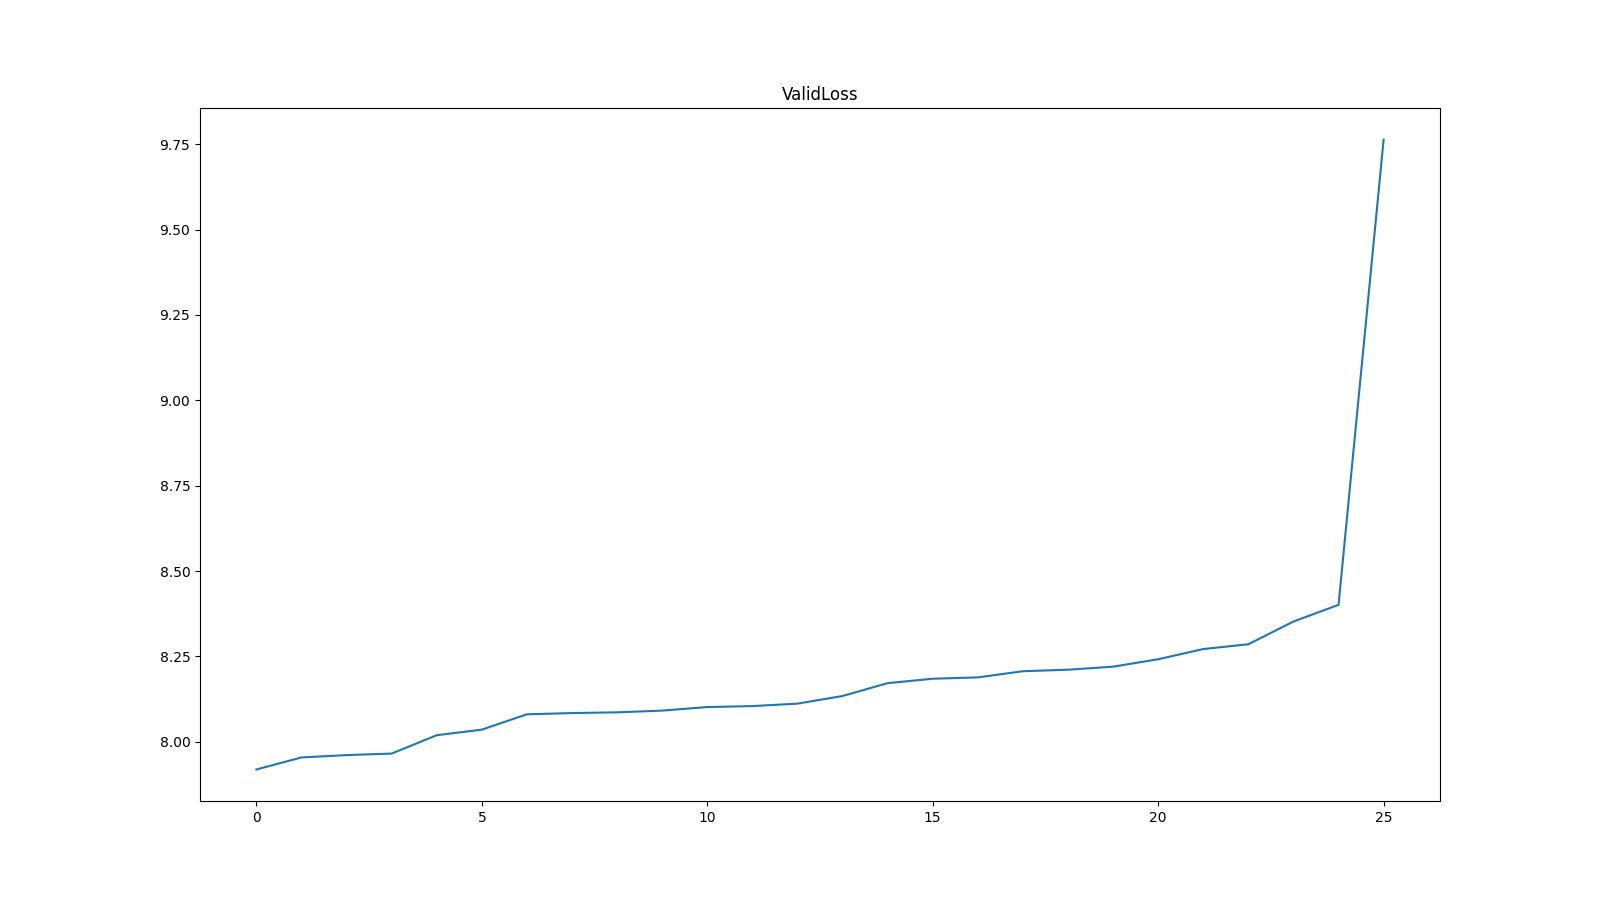
\includegraphics[scale=0.4]{./images/mixup_position/all/ValidLoss.png}
    \caption{\protect\hypertarget{image13}{Функция ошибки для всех рассматриваемых наборов позиций mixup.}}
\end{figure}

\subsection{Влияние положения Mixup}
Рассматривались положения mixup между FeatureBlock-ами, а также между последними двумя ConvBN. Точнее говоря, если описывать псевдокодом модель ResNet, рассматриваемые точки для mixup выглядят следующим образом:

\begin{lstlisting}
for i in range(5):
    x = mixup(x)                    # before_block_i
    x = self.blocks[i](x)

x = mixup(x)                        # after_blocks
x = self.final_conv1(x)
x = mixup(x)                        # after_final_conv1
x = self.final_conv2(x)
x = self.final_drop(x)
\end{lstlisting}

Основываясь на результатах \hyperlink{cite.Bas19}{[16]}, были проанализированы все варианты набора позиций для mixup, подходящие под следующие условия:
\begin{enumerate}
\item В каждом наборе присутствуют лишь 2 или 3 точки, где происходит mixup.
\item Позиции в наборе не идут последовательно друг за другом в порядке операций.
\end{enumerate}

Каждый набор позиций был проверен на части датасета размером в $N = 128'000$ образцов \hyperref[tab:mixup_position]{[Таблица 2]}. Как по всем метрикам, так и по функции ошибки, набор before-block0;before-block3 оказался наилучшим \hyperlink{image13}{[Рис 13.]} \hyperref[tab:mixup_position_metrics]{[Таблица 3]}.

\newpage
\subsection{Зависимость от количества данных}

\begin{table}[]
\centering
\begin{tabular}{||c c c c c||} 
 \hline
 type & ValidLoss & CharAcc & FragAcc & WordAcc \\ [0.5ex] 
 \hline\hline
 vanilla & 5.55 & 87.56 & 56.28 & 59.93\\ 
 \hline
 mixup & 4.85 & 88.05 & 56.87 & 60.93\\ [1ex] 
 \hline
\end{tabular}
\caption{Функция ошибки и метрики при $N = 640'000$ образцах}
\end{table}

\newpage
